\chapter{Data and Monte-Carlo Samples}\label{sec:data-and-monte-carlo-samples}

The Belle detector acquired a dataset of about $L_0 \approx 710\e{fb^{-1}}$ of integrated luminosity in its lifetime at the $\Upsilon(4S)$ energy of $10.58\e{GeV}$, which corresponds to about $771\E{6}$ $B \bar B$ meson pairs. Additionally, several streams of Monte-Carlo (MC) simulated samples were produced, where each stream of MC corresponds to the same amount of data that was recorded the detector. The main focus of work is to study a rare signal decay that is not necessarily produced abundantly or at all in the existing MC samples. In such cases, it is a common practice to produce specific samples of signal MC, where the abundance of signal decays is much larger, enabling us to study its properties in greater detail.

The following samples were used in this analysis
\begin{itemize}
	\item data
	\begin{itemize}
		\item Belle on-resonance dataset of about $L_0$ integrated luminosity, measured at $\Upsilon(4S)$ resonance energy,
		\item Belle off-resonance dataset of about $1/10 \times L_0$ integrated luminosity, measured at $60\e{MeV}$ below $\Upsilon(4S)$ resonance energy,
	\end{itemize}
	\item signal MC, corresponding to about $400 \times L_0$,
	\item other MC
	\begin{itemize}
		\item generic on-resonance, $10$ streams of $B^+B^-$ and $B^0\bar B{}^0$ (denoted as \texttt{charged} and \texttt{mixed}) and $6$ streams of $q\bar q$ produced at $\Upsilon(4S)$ resonance energy, where each stream corresponds to $L_0$,
		\item generic off-resonance, $6$ streams of $q\bar q$ produced at $60\e{MeV}$ below $\Upsilon(4S)$ resonance energy, where each stream corresponds to $1/10 \times L_0$,
		\item $B\to X_u \ell \nu$ (denoted as \texttt{ulnu}), not included in previous MC samples, equal to an amount of $20 \times L_0$, 
		\item other rare $B$ meson decays (denoted as \texttt{rare}), not included in previous MC samples, equal to an amount of $50 \times L_0$.
	\end{itemize}
\end{itemize}

\section{Signal MC Production}

The signal MC sample of $B^+ \to K^+ K^- \ell \nu_\ell$ and the charge conjugated $B^-$ decays was produced using the \texttt{mcproduzh} \cite{lange2001evtgen,agostinelli2003geant4} package for producing Belle MC. The package accepts a decay file, which describes the decays to be generated. The decay file used for signal MC generation was the same as for the \texttt{ulnu} sample since it includes the decays of interest. An additional skim was applied in order to select only events of interest with at least 2 kaons and a light lepton, all coming from the same particle. This decreases the CPU consumption during the detector simulation and reconstruction.

The relevant processes which contribute to our signal decay are
\begin{itemize}
	\item $B^+ \to a_{00} \ell^+ \nu_\ell$,
	\item $B^+ \to a_{20} \ell^+ \nu_\ell$,
	\item $B^+ \to f_{2} \ell^+ \nu_\ell$,
	\item $B^+ \to f_{0} \ell^+ \nu_\ell$,
	\item $B^+ \to X_{u}^0 \ell^+ \nu_\ell$,
\end{itemize}
where $a_{00}$, $a_{20}$, $f_{2}$ and $f_{0}$ are light unflavored states which include further decays into a $K^+K^-$ pair, and $X_u^0$ represents a generic $u \bar u$ quark pair, which further hadronizes based on the \texttt{PYTHIA} quark hadronization model \cite{sjostrand2006pythia}. Figure \ref{fig:KKsrc} shows the invariant mass of the $KK$ pair from various contributions of the MC generator. The light unflavored states have small contributions with resonant structures, while $KK$ pairs from the $X_u^0$ state are more frequent and follow a wider and smoother distribution.

\begin{figure}[H]
	\centering
	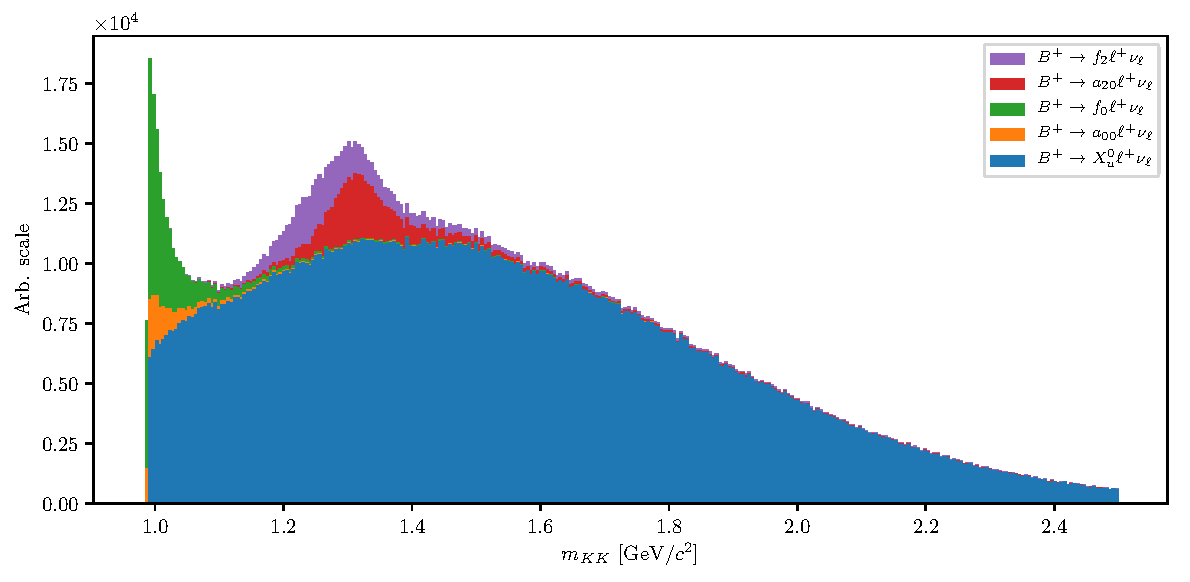
\includegraphics[width=\linewidth]{fig/KKlnu_src}
	\captionsetup{width=.8\linewidth}
	\caption{Invariant mass of the $KK$ pair from various contributions of the MC generator. The light unflavored states have small contributions with resonant structurer, while $KK$ pairs from the $X_u^0$ state are more frequent and follow a wider and smoother distribution.}
	\label{fig:KKsrc}
\end{figure}

The produced signal MC sample contains decays of the form $B \to KK\ell \nu$ as well as $B \to KKX\ell \nu$, where $X$ can be any hadron as long as it satisfies all the selection rules of the decay. It is possible to calculate the MC branching ratios for each channel by making combinations of the particles directly from the generator. Table \ref{tab:KKX} shows some of the most prominent channels, which are similar to our signal decay, as well as their relative fraction. It is clear that our signal decay is the most abundant one, with a relative contribution of about $28~\%$, while other channels contribute only up to about $8~\%$ or less. Additionally, our signal decay is the cleanest, while other decays include neutral particles like $\pi^0$, which are harder to reconstruct and suffer from a decrease in efficiency due to reconstruction effects.
\begin{table}[H]
	\centering
	\begin{tabular}{l|c||l|c}
		Channel & Ratio $[\%]$ & Channel & Ratio $[\%]$ \\
		\toprule 
		$K^+ K^-$ & 28.14 & $K^+ K^- \rho^0$ & 1.93 \\
		$K^+ K^- \pi^0$ & 8.94 & $K^+ \bar{K}{}^0 \rho^-$ & 1.84 \\
		$K^+ \bar{K}{}^0 \pi^-$ & 8.71 & $K^0 K^- \rho^+$ & 1.83 \\
		$K^0 K^- \pi^+$ & 8.70 & $K^0 \bar K {}^0 \rho^0$ & 0.00 \\
		$K^+ K^- \pi^+ \pi^-$ & 4.15 &  $K^+ K^- \pi^0 \pi^0$ & 0.86 \\
		$K^0 \bar K {}^0$ & 3.32  & $K^+ K^- \pi^+ \rho^-$ & 0.69 \\
		$K^0 \bar K {}^0 \pi^0$ & 3.26 & $K^+ K^- \rho^+ \pi^-$ & 0.68 \\
		\midrule
		$K \bar K$ pair with $\eta$ & 7.08  & & \\
		$K \bar K$ pair with $\omega$ & 5.33  & & \\
		Other & 14.53  & & \\
		\bottomrule 
	\end{tabular}
	\captionsetup{width=.8\linewidth}
	\caption{Relative branching ratios of $B \to KKX\ell \nu$ decays by channel.}
	\label{tab:KKX}
\end{table}

We generate about $1.3\E{9}$ events of the form $B\to X_u \ell \nu$, which corresponds to an integrated luminosity of about $L = 400\times L_0$, where this value was obtained by normalizing the signal MC to the amount of signal in the $B\to X_u \ell \nu$ MC sample. This amounts to a total of about $9.37\E{6}$ generated signal events, and to a branching ratio
\begin{equation}
\mathcal{B}\left(B^+ \to K^+ K^- \ell^+ \nu_\ell\right)_{MC} = 1.53\E{-5},
\end{equation}
where $\ell$ is $e$ or $\mu$. During analysis, the abundant signal MC sample is scaled down to correspond to the amount of data taken with the Belle detector.

\section{Control Decay}\label{sec:control-decay}

In this analysis, we are also able to define another $B$ meson decay which occupies almost the same phase space as our signal decay. This process can be used for the monitoring of our analysis steps, which are applied to both measured and simulated data. Any kind of difference between the two might indicate our procedure to be fine-tuned to simulated data, or some other similar problem. 

We define a control decay of the form $$B^+ \to \bar D {}^0 \ell^+ \nu, \quad D^0 \to K^+ K^-,$$ which is much more abundant and, most importantly, easy to suppress since it only populates a very narrow region in the kaon invariant mass spectrum. Due to no extra particles in the $D^0$ decay, the kaon invariant mass is equal to $m_{KK} \approx m_{D^0}$ up to very good precision. By excluding this narrow region we discard the majority of the control candidates while discarding only a small amount of the signal candidates. A more quantitative description of suppressing control and other background candidates is written in Chapter \ref{sec:background-suppression}.